%%%%%%%%%%%%%%%%%%%%%%%%%%%%%%%%%%%%%%%%%%%%%%%%%%%%%%%%%%%%%%%%%%%%%%%%%%%%%%%%
% Preámbulo                                                                    %
%%%%%%%%%%%%%%%%%%%%%%%%%%%%%%%%%%%%%%%%%%%%%%%%%%%%%%%%%%%%%%%%%%%%%%%%%%%%%%%%

\documentclass[11pt,a4paper,titlepage,twoside,openright,openbib]{report}

%%% RELACIÓN DE VARIABLES A PERSONALIZAR %%%
\def\lingua{gal}
%\def\lingua{esp} % descomenta esta liña se redactarás a memoria en español
%\def\lingua{eng} % descomenta esta liña se redactarás a memoria en inglés
\def\nomeA{Xico Fernández Lozano (\href{mailto:xico.fernandez@udc.es}{xico.fernandez})}
\def\nomeB{Mario Páez Marcote (\href{mailto:mario.paez@udc.es}{mario.paez})}% substitúe aquí o teu nome
\def\nomeC{Andrés Filipe Oliveira da Silva (\href{mailto:andres.oliveira@udc.es}{andres.oliveira})}             % substitúe aquí o nome de quen dirixe
\def\titulo{XOGO DO FORCADO PARA ANDROID  ForcApp}

\def\icon{\begin{figure}[hp!]
  \centering
  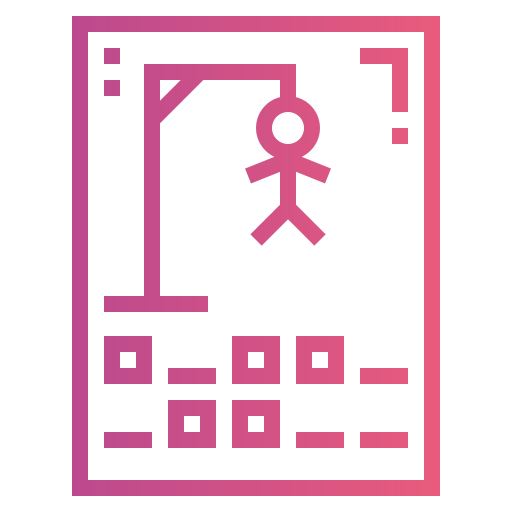
\includegraphics[width=0.15\textwidth]{imaxes/icon.png}
  \label{fig:icon}
\end{figure}}


%\def\mencion{COMPUTACIÓN}
%\def\mencion{ENXEÑARÍA DO SOFTWARE}
\def\mencion{ENXEÑARÍA DE COMPUTADORES}
%\def\mencion{SISTEMAS DE INFORMACIÓN}
%\def\mencion{TECNOLOXÍAS DA INFORMACIÓN}

%\def\renomearcadros{si} % descomenta esta liña se redactas a memoria en español e prefires que
                         % os "cuadros" e o "índice de cuadros" se renomeen
                         % a "tablas" e "índice de tablas" respectivamente

\usepackage{estilo_tfg}
  
% Lista de paquetes potencialmente interesantes (uso baixo demanda)

% \usepackage{alltt}       % proporciona o entorno alltt, semellante a verbatim pero que respecta comandos
% \usepackage{enumitem}    % permite personalizar os entornos de lista
% \usepackage{eurofont}    % proporciona o comando \euro
% \usepackage{float}       % permite máis opcións para controlar obxectos flotantes (táboas, figuras)
% \usepackage{hhline}      % permie personalizar as liñas horizontais en arrays e táboas
% \usepackage{longtable}   % permite construir táboas que ocupan máis dunha páxina
% \usepackage{lscape}      % permite colocar partes do documento en orientación apaisada
% \usepackage{moreverb}    % permite personalizar o entorno verbatim
% \usepackage{multirow}    % permite crear celdas que ocupan varias filas da mesma táboa
% \usepackage{pdfpages}    % permite insertar ficheiros en PDF no documento
% \usepackage{rotating}    % permite diferentes tipos de rotacións para figuras e táboas
% \usepackage{subcaption}  % permite a inclusión de varias subfiguras nunha figura
% \usepackage{tabu}        % permite táboas flexibles
% \usepackage{tabularx}    % permite táboas con columnas de anchura determinada

%%%%%%%%%%%%%%%%%%%%%%%%%%%%%%%%%%%%%%%%%%%%%%%%%%%%%%%%%%%%%%%%%%%%%%%%%%%%%%%%
% Corpo                                                                        %
%%%%%%%%%%%%%%%%%%%%%%%%%%%%%%%%%%%%%%%%%%%%%%%%%%%%%%%%%%%%%%%%%%%%%%%%%%%%%%%%

\begin{document}

 %%%%%%%%%%%%%%%%%%%%%%%%%%%%%%%%%%%%%%%%
 % Preliminares do documento            %
 %%%%%%%%%%%%%%%%%%%%%%%%%%%%%%%%%%%%%%%%

 \begin{titlepage}
  
  \hspace*{128pt}
  \textcolor{udcpink}{{\fontencoding{T1}\fontfamily{phv}\selectfont Facultade de Informática}}\\[-32pt]

  \begin{center}
    
\includegraphics[scale=0.3]{imaxes/udc}\\[35pt]

    {\large PROGRAMACIÓN DE SISTEMAS \\
            Primeiro Cuadrimestre 2021/22
           } \\[50pt]
    
    \begin{huge}
      \begin{spacing}{1.3}
        \bfseries \titulo \\ 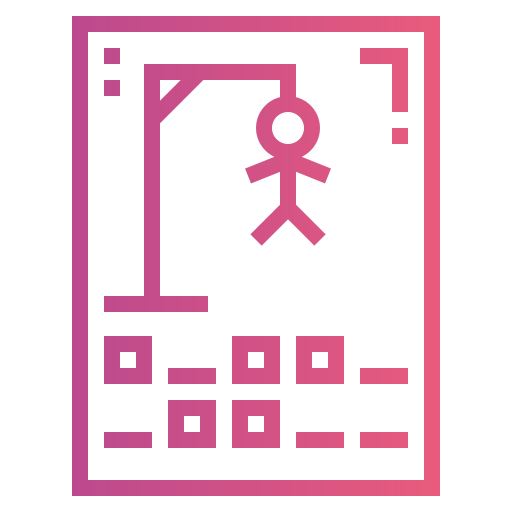
\includegraphics[scale=0.6]{imaxes/icon.png}\\[35pt]
      \end{spacing}
    \end{huge}
  \end{center}
  
  \vfill
  
  \begin{flushright}
    {\large
    \begin{tabular}{ll}
      {\bf Estudante:} & \nomeA \\
      {\bf Estudante:} & \nomeB \\
      {\bf Estudante:} & \nomeC \\ % COPIA E PEGA ESTA LIÑA MÁIS VECES SE O PRECISAS
    \end{tabular}}
  \end{flushright}
  \rightline{A Coruña, \datasimple\today. Versión 0.3}
\end{titlepage}

 \pagenumbering{roman}
 \setcounter{page}{1}
 \bstctlcite{IEEEexample:BSTcontrol}

\begin{table}[h!]
\centering
\begin{tabular}{||c | c||} 
 \hline
 \textbf{Versión} & \textbf{Data}\\ [0.5ex] 
 \hline\hline
 0.1 & 04/10/2021\\
  [1ex] 
 \hline
 0.2 & 08/11/2021\\
  [1ex] 
 \hline
 0.3 & 13/01/2021\\
  [1ex] 
 \hline
  0.4 & 15/01/2022\\
  [1ex] 
 \hline
 0.5 & 18/01/2022\\
  [1ex] 
 \hline
\end{tabular}
\caption{Táboa coas versións do proxecto.}
\label{table:1}
\end{table}

\let\cleardoublepage=\clearpage 

 \tableofcontents
% \listoffigures
% \listoftables

\vspace{30pt}


 %\cleardoublepage
 
 

 \pagenumbering{arabic}
 \setcounter{page}{1}
 
  \chapter{Introdución}
\label{chap:introducion}
\section{Obxetivos}
Este proxecto consiste en elaborar un xogo para o sistema operativo \textbf{ANDROID} basado no tradicional xogo do \textbf{Forcado}. O obxetivo da aplicación é poder xogar de maneira \textbf{individual} ou \textbf{multixogador} tratando de adiviñar a palabra secreta antes de que se forme por completo o forcado.\\
Como obxetivo principal, está no desenvolvemento da aplicación para poder xogar de maneira local, é dicir, dende unha soa terminal.
Logo, estudiarase a opción de poder xogar online a través dos distintos terminais interconectados entre sí.
\section{Motivación}
Elixiuse implementar este tipo de xogos despois de estudar a demanda na Play Store. Os xogos de entretemento como os naipes, xadrez, parchís... Dispón de moitas descargas na Play Store e o seu desenvolvemento é mais doado que outras aplicacións deseñadas por grandes compañías.


\section{Traballo relacionado}
Hai diversas aplicacións na Play Store nas que desenvolveron o mesmo xogo.
As dúas con maior impacto a nivel de descargas (> 10 millóns), e polo tanto, nas que nos estamos baseando, son as seguintes:\\
\href{https://play.google.com/store/apps/details?id=com.tellmewow.senior.hangman&hl=es&gl=US}{Ahorcado desarrollado por Senior Games}\\
\href{https://play.google.com/store/apps/details?id=com.quarzo.hangmanwords&hl=es&gl=US}{Ahorcado desarrollado por Quarzo Apps}

 \let\cleardoublepage=\clearpage 


 \chapter{Análisis de requisitos}
\label{chap:requisitos}
\section{Funcionalidades}
Esta aplicación dispoñerá de catro funcionalidades principais:
\begin{itemize}

    \item \textbf{Menú principal}: Funcionalidade "de enlace" co resto das funcionalidades. É a base da aplicación.
    
    \item \textbf{Dicionario}: Apoiarase nunha base de datos deseñada con \textit{Room} para gardar as palabras e poder seleccionar unha aleatoriamente á hora de comezar unha partida. Poderanse eliminar e engadir palabras. Non se permitirá utilizar o dicionario baleiro no resto de funcionalidades. Non se poderá introducir unha palabra maior a 17 caracteres por cuestión de espazo. Haberá comprobación dos caracteres introducidos.
    
    \item \textbf{Modo un xogador}: Esta funcionalidade consistirá en permitir ao usuario poder xogar de maneira individual. Neste caso, a aplicación escollerá unha palabra aleatoria dende un dicionario (podendo ser este ampliable polos usuarios) situado nos propios arquivos da aplicación e presentaralla ao usuario por pantalla para que trate de adiviñala. Ademais a aplicación amosará un teclado 'artificial' sen necesidade de usar un do sistema. Ao seleccionar unha letra dese teclado amosarase sombreada e non será posible volver a seleccionala.
    
    
    \item \textbf{Modo multixogador}: Nesta funcionalidade permitirase a dous usuarios xogar un contra outro. O funcionamento segue o mesmo modo que o dun xogador (hereda a súa vista) pero cun contador no que se amosa o tempo restante para elexir unha letra. Se este tempo expira, o xogador será eliminado. Gañará o xogador que adiviñe antes a palabra para evitar situacións de empate ou o que quede sen ser eliminado. Esta funcionalidade encárgase da parte de autencicación de usuarios e comunicacións en liña. Será necesario engadir todo o proceso de autentificación e unha sala de espera virtual para iniciar a partida cando os dous xogadores se presenten como listos.
    
\end{itemize}
\begin{center}
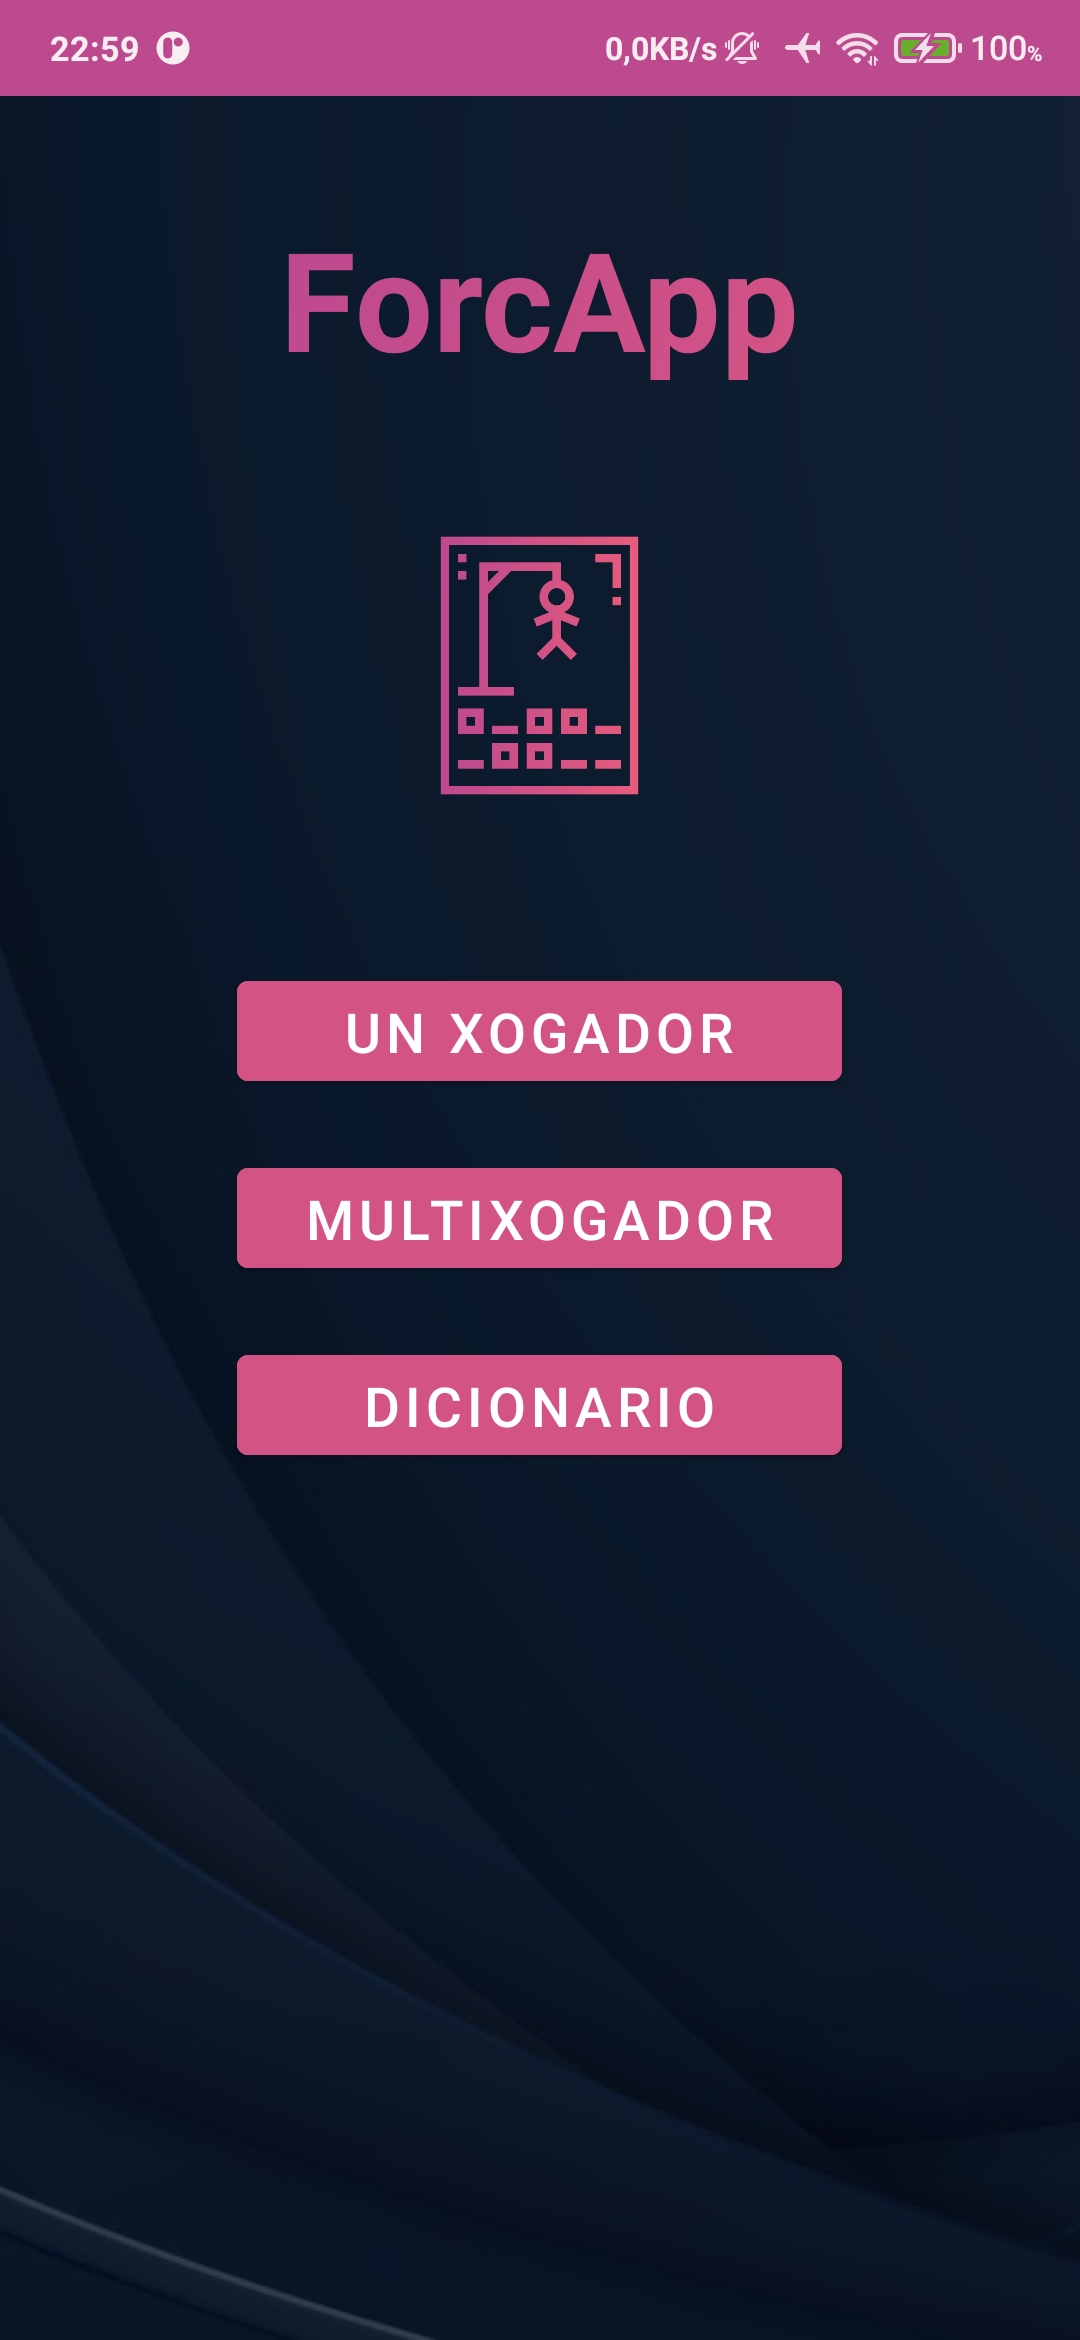
\includegraphics[scale=0.105]{imaxes/menu.jpg}
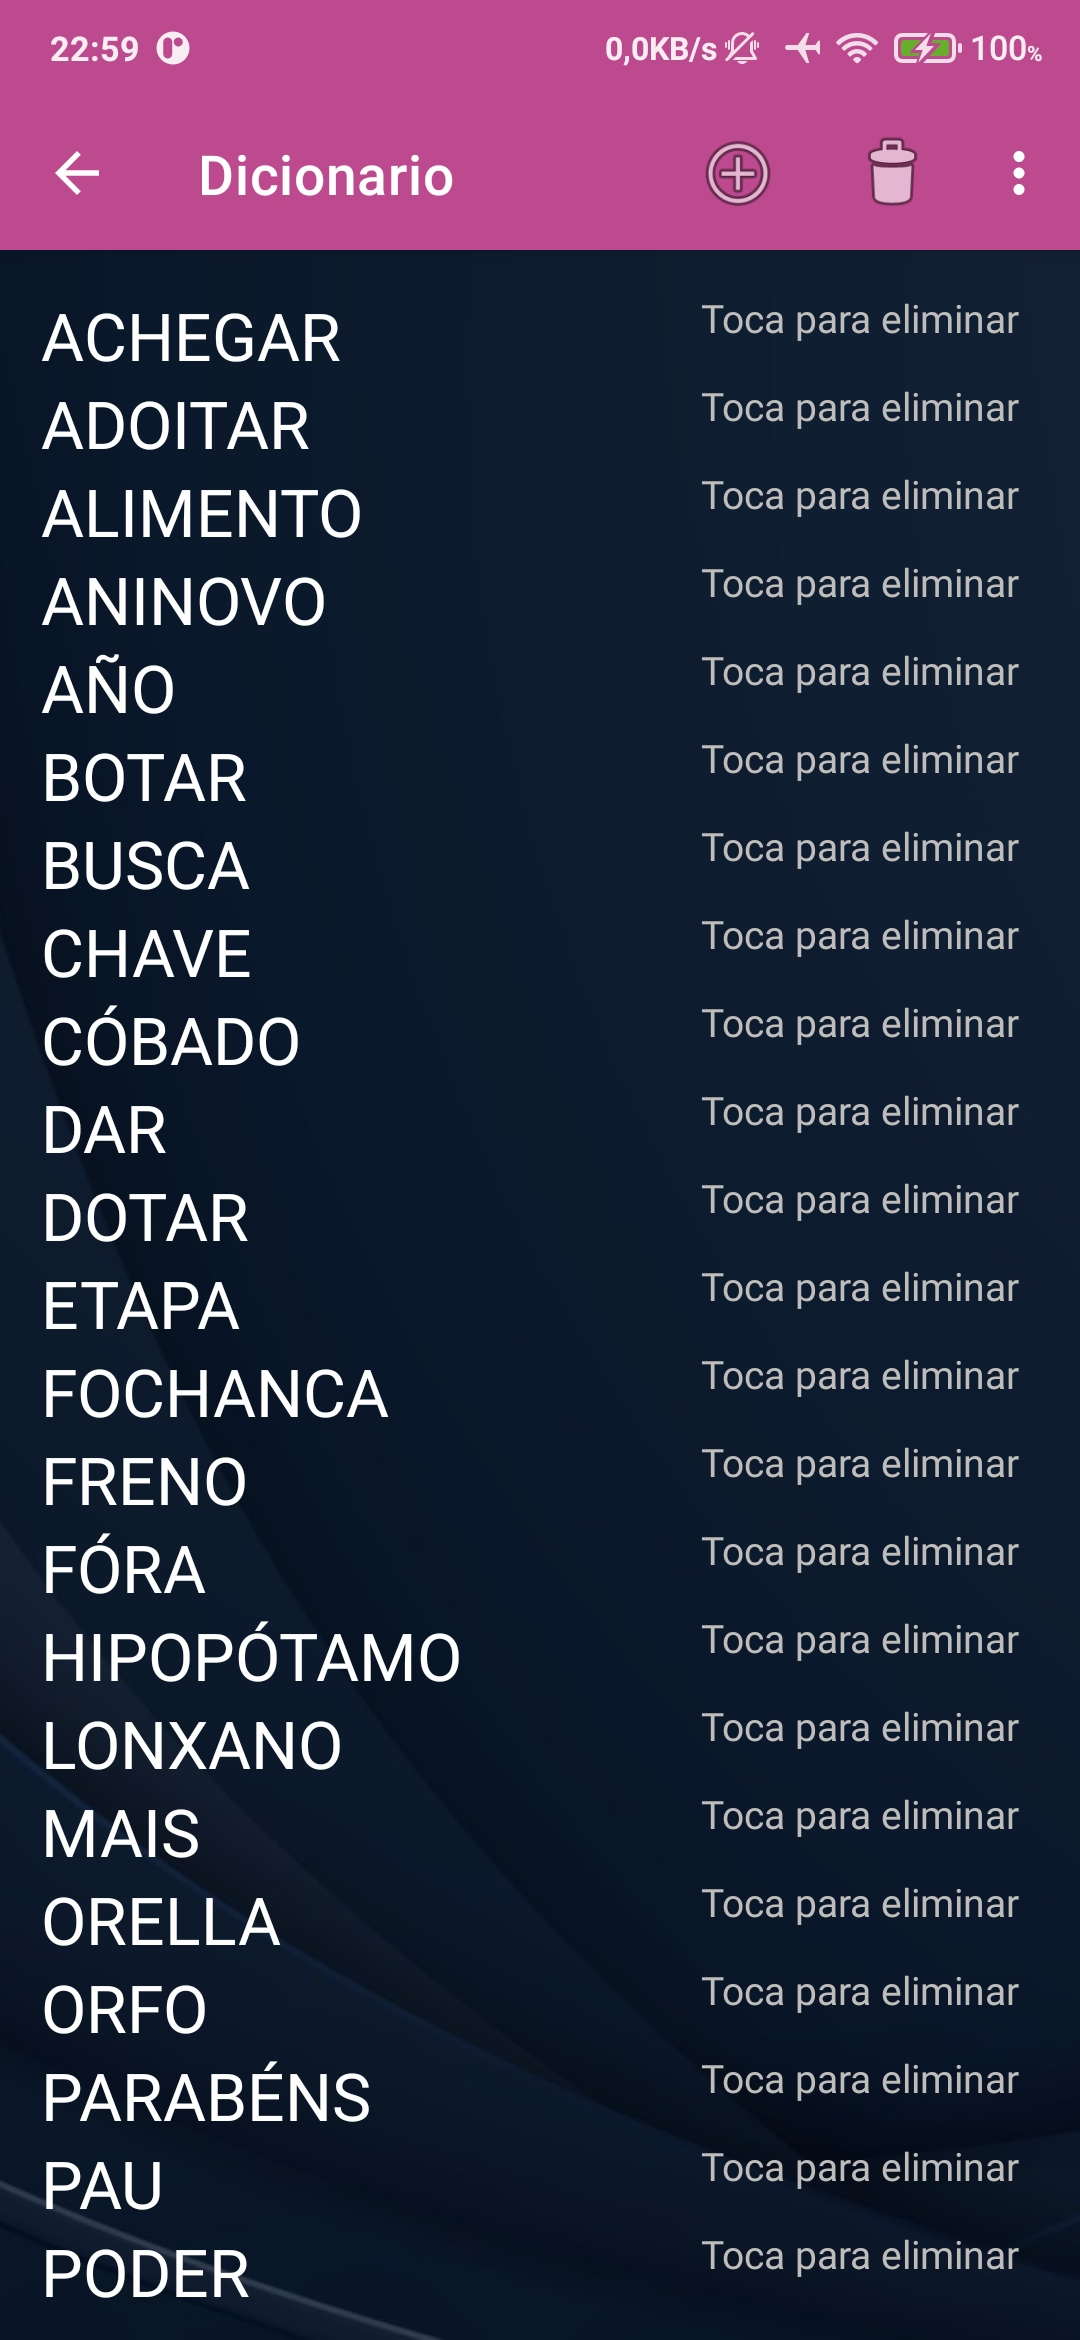
\includegraphics[scale=0.105]{imaxes/dicionario.jpg}
\end{center}
\begin{center}
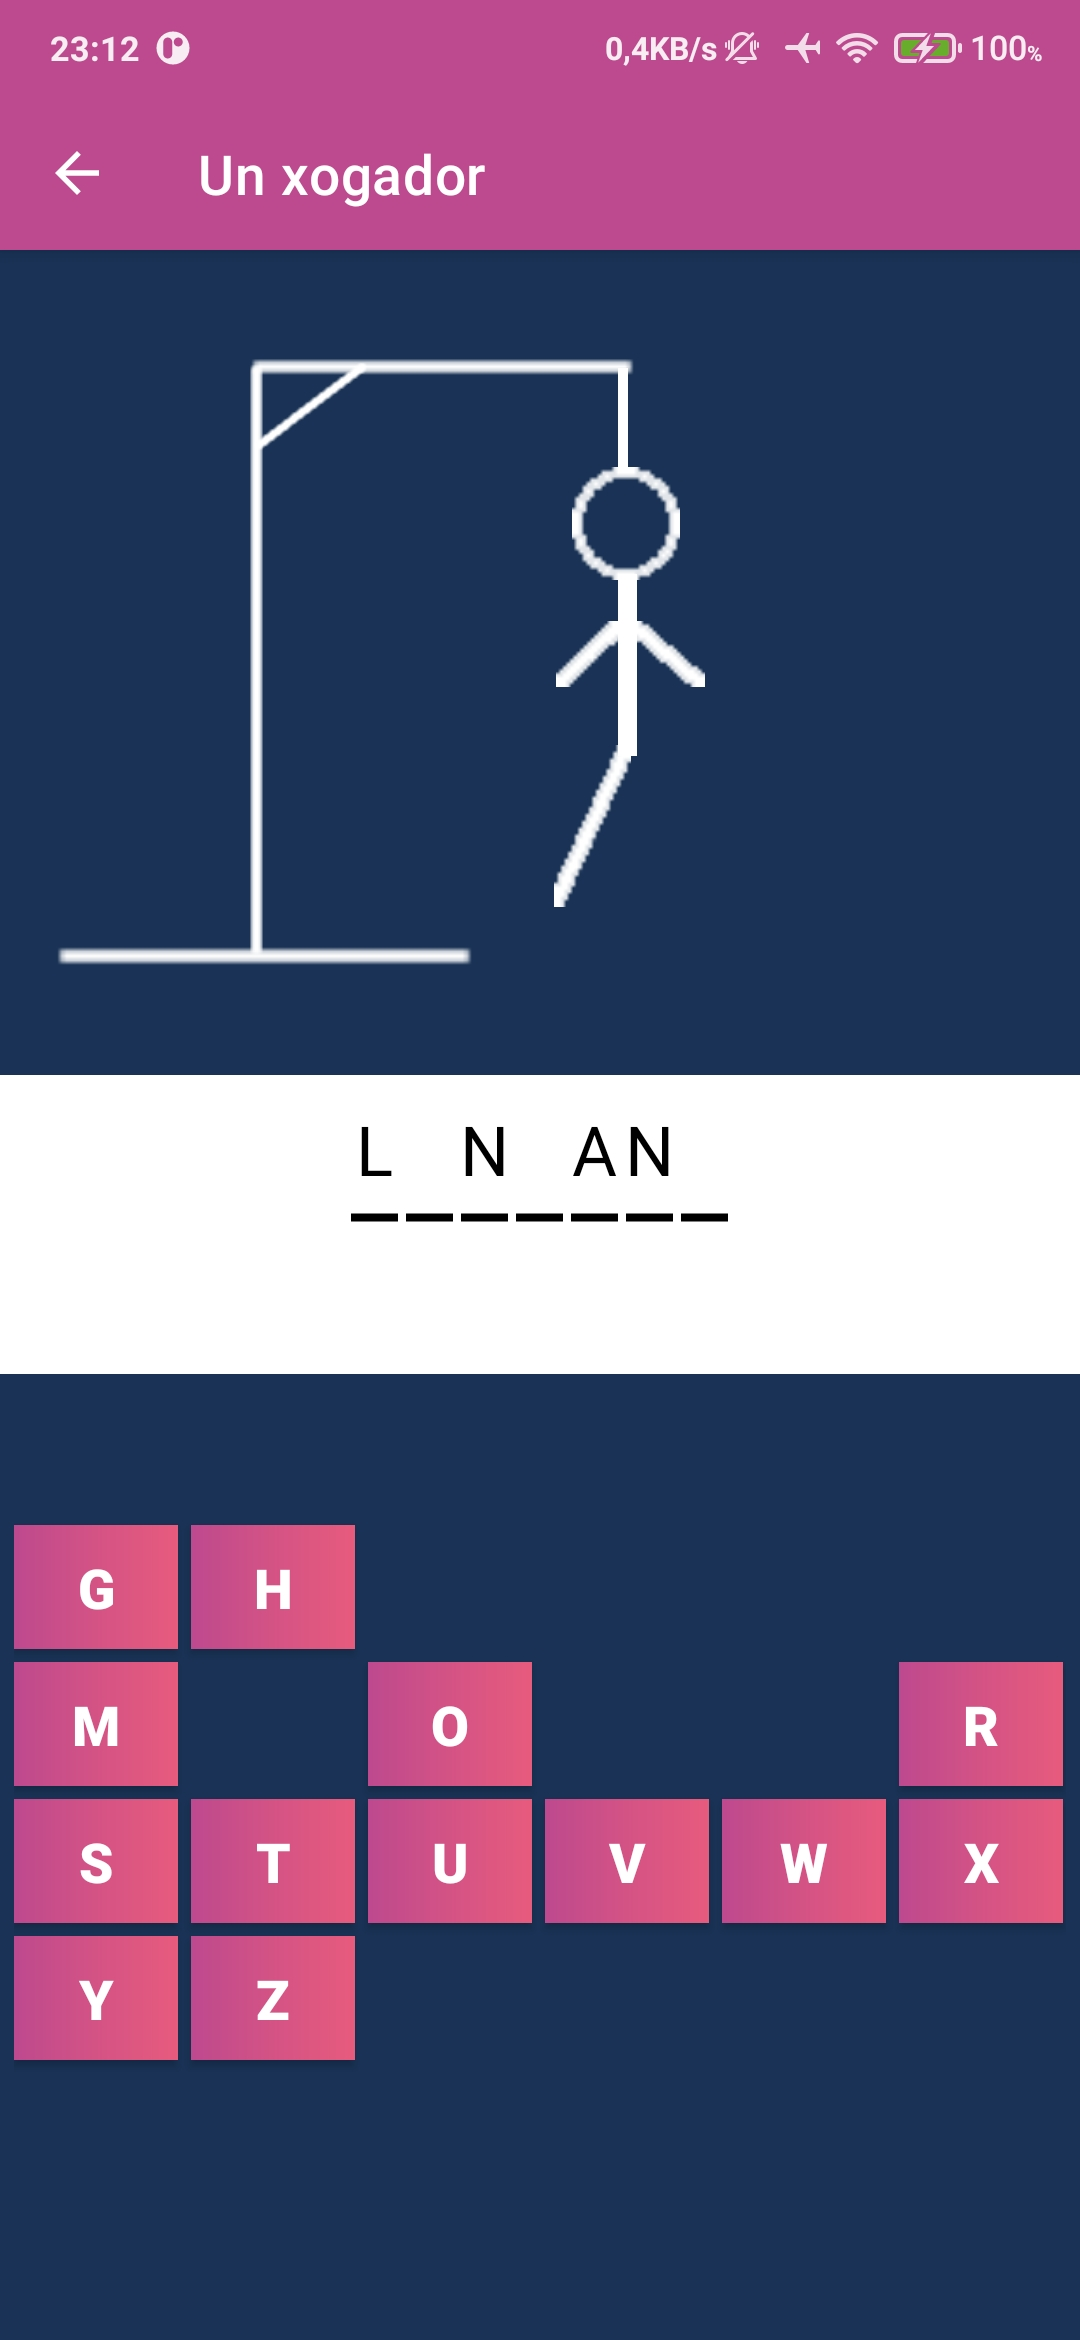
\includegraphics[scale=0.105]{imaxes/singleplayer.jpg}
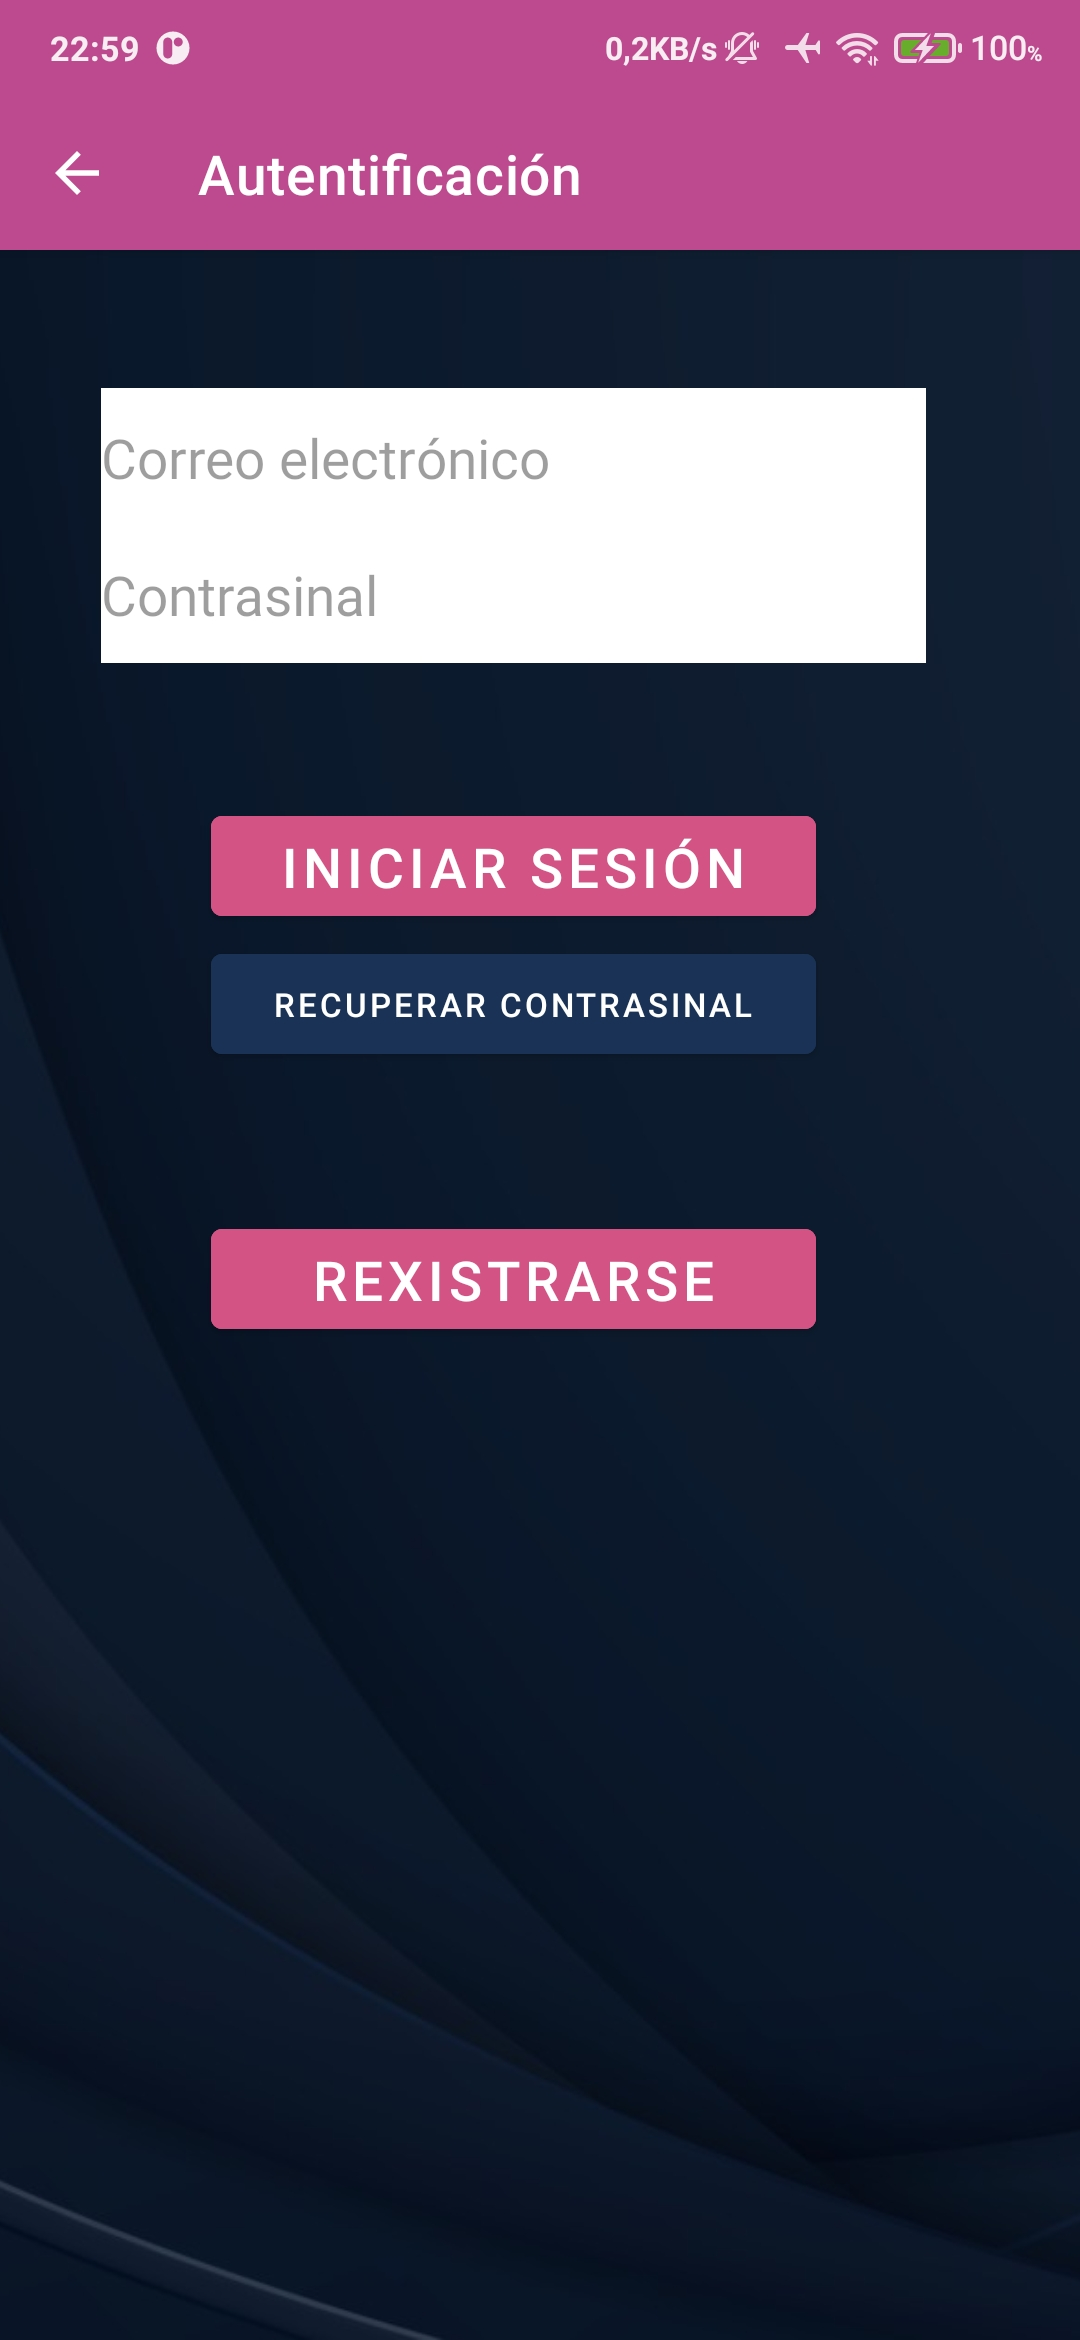
\includegraphics[scale=0.105]{imaxes/auth.jpg}\\[30 pt]
\end{center}
A prioridade de implementación das funcionalidades seguirá a orde descrita anteriormente, sendo o menú principal a primeira funcionalidade en ser implementada, o modo multixogador o último.\\
\section{Traballos futuros}
En traballos futuros pódense engadir novas funcionalidades como levar a conta de partidas gañadas e perdidas (pódense calcular estatísticas como porcentaxes de éxito ou número de intentos medios para obter unha victoria) en calquera dos dous modos, para isto faría falta outra base de datos a maiores, por último conviría desenvolver un multixogador en liña para máis de dous xogadores.\\
\\
Plantexamos elaborar tamén un proceso de testeo da aplicación coa axuda de usuarios e distintos tipos de probas de validación do software. Se se chegase a distribuír a aplicación cumpriría mantela con parches e actualizacións.

Tamén se considera a idea de seguir un modelo para o software da aplicación como pode ser o MVC que separa a vista do modelo mediante un controlador. Sería importante engadir soporte para diferentes idiomas e dispositivos en función da súa pantalla e do tamaño de fonte definido polo usuario a nivel de sistema operativo. De momento solo está pensado para estes parámetros en modo predeterminado.
 \let\cleardoublepage=\clearpage 
 \chapter{Planificación Inicial}
\label{chap:plan_inicial}

\section{Iteracións}
O proxecto fragmentarase na iteración de presentación do proxecto (\textit{brainstorming}, preparación dos documentos necesarios), as tres primeiras funcionalidades \textit{offline} a o multixogador \textit{online} por últimno. Como iteracións complementarias están os traballos futuros e as probas de validación do software.

\section{Responsabilidades}
Por dispoñibilidade temporal, a idea é que todos os integrantes do grupo implementen as funcionalidades xuntos xa que é improbable que se solapen os traballos de dous recursos diferentes.\\
\\
Tódolos membros do grupo terán a mesma porcentaxe de responsabilidade aínda que o esperable é que os traballos se vaian asignando dinamicamente e sobre a marcha do proxecto segundo sexa necesario.\\
\\
Botaremos man do control de versións \textit{git} utilizando \textit{GitFlow} definindo as diferentes ramas para facilitar o traballo. Crearase unha rama \textit{latex} exclusiva para gardar o código fonte da elaboración deste \textit{PDF} e o documento en si.

\section{Fitos e entregables}
Haberá un total de 2
fitos, un para cada unha das funcionalidades a realizar cada unha cun mes de duración. Primeiro farase o modo dun xogador e todo o que conleva (dicionario e menú principal), facer todas as vistas e código para que se poida xogar con normalidade. Este punto marcará o fin do primeiro fito.\\
\\
No segundo , partiremos do traballo xa relaizado para elaborar a lóxica e as vistas do modo multixogador, ao estar rematado darase por finalizado o segundo fito.


\section{Incidencias e plans de continxencia}
O principal risco que se vai ter en conta en conta debido á súa probable materialización son os contratempos á hora do desenvolvemento \textit{software} e resolución de \textit{bugs}. Este risco está presente en case todos os proxectos \textit{software} e aínda máis cando se trata dun proxecto non profesional e con falta de experiencia na metodoloxía.\\
\\
A solución aplicada para isto é tratar de adiantar o proxecto máximo posible coa mentalidade pesimista de que chegará algún contratempo que retrase o proceso.\\
\\
Para a solución de \textit{bugs} na interface intentaranse forzar as funcionalidades da aplicación o máximo posible e intentar solucionalos modificando o código. Para a solución de excepcións da linguaxe (\textit{Java} e \textit{xml}) botaremos man do \textit{debugger} para ver os valores dos datos da aplicación en cada momento e ver o que sucede en cada intre para distintos valores. Para verificar o correcto funcionamento da base de datos utilizarase a funcionalidade \textit{App Inspector} incorporada en \textit{Android Studio}.\\
\\
Como incidencias destacables ganaron importancia a xestión do cambio de tema (entre escuro e claro) do sistema operativo xa que daba lugar a basantes \textit{bugs} e a concurrencia á hora de acceder a un resultado que se necesitaba de inmediato durante unha consulta a \textit{Firebase}.

 \let\cleardoublepage=\clearpage 
  \let\cleardoublepage=\clearpage 
 \include{contido/deseño}
  \let\cleardoublepage=\clearpage 

 %%%%%%%%%%%%%%%%%%%%%%%%%%%%%%%%%%%%%%%%
 % Capítulos                            %
 %%%%%%%%%%%%%%%%%%%%%%%%%%%%%%%%%%%%%%%%


 %%%%%%%%%%%%%%%%%%%%%%%%%%%%%%%%%%%%%%%%
 % Apéndices, glosarios e bibliografía  %
 %%%%%%%%%%%%%%%%%%%%%%%%%%%%%%%%%%%%%%%%

 %\appendix
 %\appendixpage
 %\chapter{Material adicional}
\label{chap:adicional}

\lettrine{E}{xemplo} de capítulo con formato de apéndice, onde se pode
incluír material adicional que non teña cabida no corpo principal do
documento, suxeito á limitación de 80 páxinas establecida no
regulamento de TFGs.

\Blindtext

%\include{anexos/...}

 %\printglossary[type=\acronymtype,title=\nomeglosarioacronimos]
% \printglossary[title=\nomeglosariotermos]

 \bibliographystyle{IEEEtranN}
 \bibliography{\bibconfig,bibliografia/bibliografia}
  \let\cleardoublepage=\clearpage 
 
\end{document}

%%%%%%%%%%%%%%%%%%%%%%%%%%%%%%%%%%%%%%%%%%%%%%%%%%%%%%%%%%%%%%%%%%%%%%%%%%%%%%%%
